% Created 2021-08-11 mié 22:36
% Intended LaTeX compiler: pdflatex
\documentclass[11pt]{article}
\usepackage[utf8]{inputenc}
\usepackage[T1]{fontenc}
\usepackage{graphicx}
\usepackage{grffile}
\usepackage{longtable}
\usepackage{wrapfig}
\usepackage{rotating}
\usepackage[normalem]{ulem}
\usepackage{amsmath}
\usepackage{textcomp}
\usepackage{amssymb}
\usepackage{capt-of}
\usepackage{hyperref}
\author{Jonatan Ahumada \& Jorge Garzón}
\date{\today}
\title{Becos}
\hypersetup{
 pdfauthor={Jonatan Ahumada \& Jorge Garzón},
 pdftitle={Becos},
 pdfkeywords={},
 pdfsubject={},
 pdfcreator={Emacs 27.2 (Org mode 9.4.4)}, 
 pdflang={English}}
\begin{document}

\maketitle
\tableofcontents



\section{Análisis del entorno}
\label{sec:orgb5b8dd2}
\subsection{PESTEL}
\label{sec:org09f5649}
\subsubsection{Político}
\label{sec:orga4b85a3}
\begin{enumerate}
\item Amenaza de variante delta
\label{sec:orgd4d9a0e}

Con la aparición de la variante delta, la comunidad internacional está
considerando volver a implementar medidas de aislamiento.

Esto es una \textbf{amenaza} porque la infraestructura física requiere un
plantel de trabajadores para sus procesos de confección, que está
ligado a la mano de obra de las trabajadoras. Habra más costos para
garantizar la salubridad y hay límites de espacio que se deben
respetar, lo que disminuye capacidad de producción

\item Cese de presencialidad en los colegios
\label{sec:org9913e54}

Si se prolonga el aislamiento social, por un posible cuarto pico, la
proyección de ventas se desploma, puesto que prinipalmente recae en
escuelas de futbol y colegios de Bogotá, que participan en torneos
locales.

Esto es una \textbf{amenaza} porque no habrá demanda de uniformes.

\item Déficit fiscal y tributación de la reforma 2.0:
\label{sec:org4bb4264}

En la nueva reforma fiscal la tarifa de renta subirá del 30 al 35\%
para hacerle frente al déficit fiscal que enfrenta el país.

Esto es una \textbf{amenaza} porque los márgenes de rentabilidad será más
estrecho.  Más aun, teniendo en cuenta el costo competitivo que el
plan de negocios plantea para sus productos.
\end{enumerate}

\subsubsection{Económico}
\label{sec:orga1c8f58}
\begin{enumerate}
\item Alsa del dólar
\label{sec:orgb580210}
La amenaza de la variante delta hace que la Fed aumente las tasas de
interés del dolar, lo que desvaloriza el peso colombiano frente a la
divisa.

Esto es una \textbf{amenaza} porque puede disuadir la inversión.

\item Proceso de reactivación económica
\label{sec:org9d45ccf}
\end{enumerate}
\subsubsection{Social}
\label{sec:org3c12fed}
\begin{enumerate}
\item Protagonismo del sector textil colombiano a nivel internacional
\label{sec:org3401d7b}

El sector textil y la moda registra el 37\% de las empresas registrados
en CCB.  Según Colombia productiva, el sector textil y de confección
es el primer generador de mano de obra en la industria
nacional. Además, colombia es el primer exportador de tejido plano en
Suramérica.

Esto es una \textbf{oportunidad} porque el reconocimiento externo de la moda
colombiana podría potenciar aún más la propuesta diferenciadora de
Becos: ayudar a madres cabezas de hogar de sectores vulnerables a la
vez que se contrinuye al medio ambiente.

\item Necesidad de impulsar la reactivación económica
\label{sec:org88df624}

El Gobierno Duque enfatiza que el pais muestra ritmo de crecimiento
elevado (1,1\%) el primer trimestre del año, en comparación con paises
como Chile o México. El gobierno pronostica un desarrollo favorable
durante el resto del año.

Esto es una \textbf{oportunidad} porque parece improbable que el gobierno
actual paralice la reactivación ecónomica, más aún si se se han hecho
esfuerzos presupuestales para iniciar le proceso de vacunación.
\end{enumerate}

\subsubsection{Tecnológico}
\label{sec:orgcf4ae6c}

\subsubsection{Ambiental}
\label{sec:org8b85af3}
\begin{enumerate}
\item Aceptación cultural del reciclaje
\label{sec:org60c89de}
El mundo está entrando en periodo de conciencia ambiental. En
Colombia, sectores como el de los hidrocarburos están iniciado una
transformación hacia energías más limpias.

Esto es una \textbf{oportunidad}, puesto que hay una tendencia cultural
por participar en la genereción de un mundo ecosostenible, lo
que hace que la propuesta de Becos altamente atractiva en el pais
y el mundo por igual.
\end{enumerate}
\subsubsection{Legal}
\label{sec:orgde209b9}
\subsection{5 Fuerzas}
\label{sec:orgce6de29}

\begin{center}
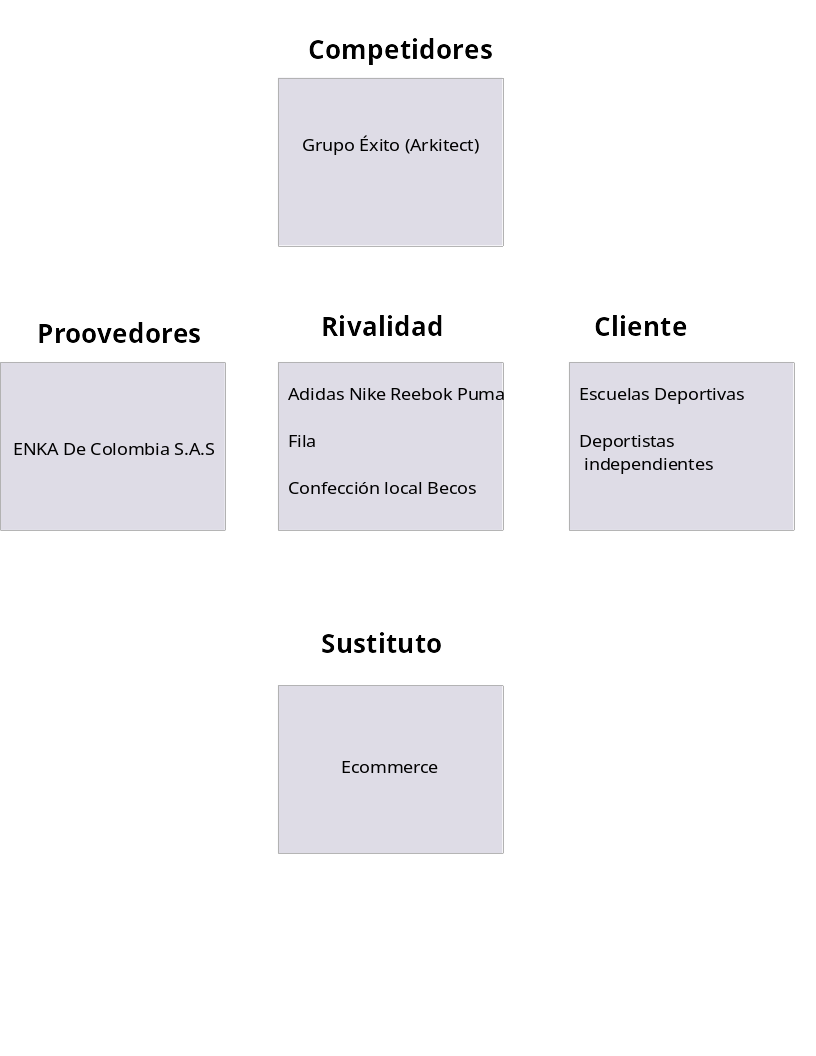
\includegraphics[width=.9\linewidth]{./assets/build/5_fuerzas.png}
\end{center}

\subsection{BMM}
\label{sec:org9b63dec}

\subsubsection{Assesment}
\label{sec:org0e3ea05}
\begin{enumerate}
\item Influencias
\label{sec:org3914a09}

\begin{enumerate}
\item Externas

\begin{itemize}
\item Gobierno Colombiano
\item Mercado Internacional
\item Confeccionistas de Bogotá
\end{itemize}
\end{enumerate}


\begin{enumerate}
\item Internas

\begin{itemize}
\item Adecuación a protocolos de Bioseguridad
\item Implementación de hardware y software
\end{itemize}
\end{enumerate}

\item DOFA
\label{sec:org7210582}

\begin{center}
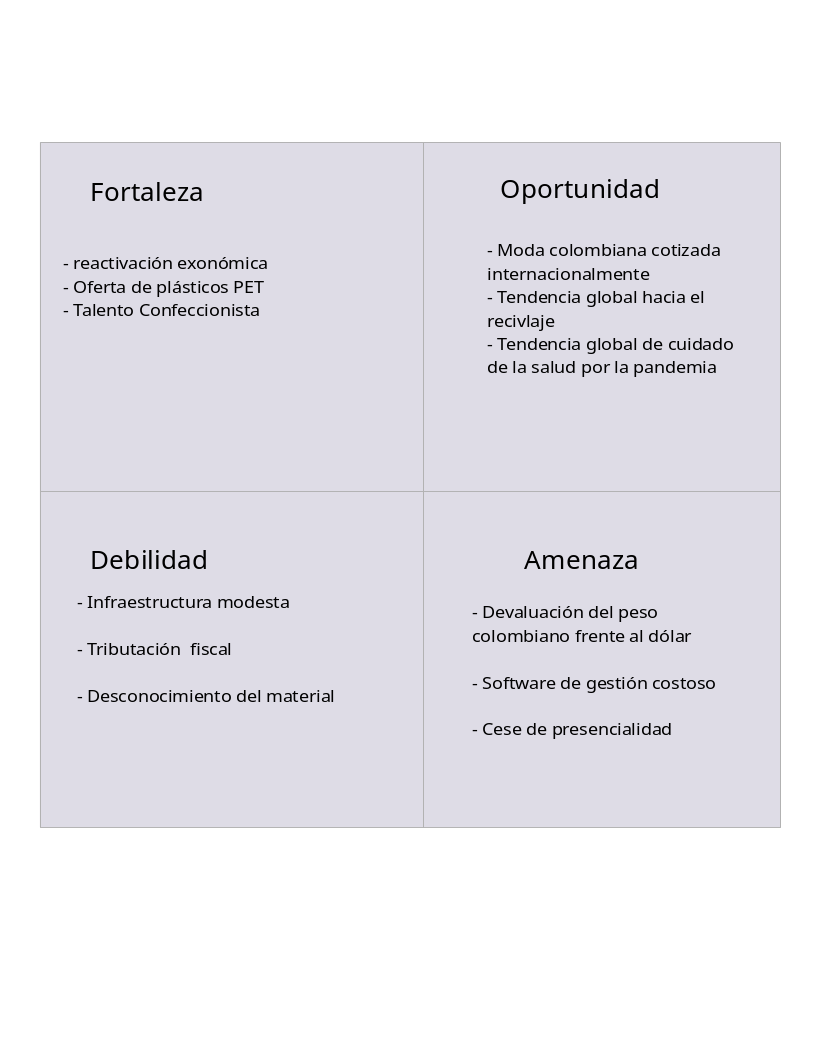
\includegraphics[width=.9\linewidth]{./assets/build/dofa.png}
\end{center}
\end{enumerate}


\subsubsection{Medios}
\label{sec:org9a5754b}

\begin{enumerate}
\item Integracion
\label{sec:orgdad2ffc}
\begin{itemize}
\item Apuntar a mercado internacional
\item Formar alianzas intenrnacionales y locales
\end{itemize}

\item Intensivas
\label{sec:org05d4567}
\begin{itemize}
\item aumentar precios de productos para mercado internacional
\item fortalecer la linea de producto personalizado
\item mayor valor agregado al proceso de confección
\end{itemize}

\item Diversificación
\label{sec:orgd1a5a4d}

\begin{itemize}
\item Aumentar catálogo de producto a mayores actividades
\item Ventas online
\end{itemize}

\item Defensivas
\label{sec:org46da924}
\begin{itemize}
\item Recortar sueldos
\item Optimizara costos operacionales
\item Solicitar subsidios y exenciones
\item Usar ERP y CRM con licencias GPL
\end{itemize}
\end{enumerate}

\subsubsection{Externas}
\label{sec:orgf7a4339}
\subsection{Blue Ocean Strategy Canvas \& ERRC GRID}
\label{sec:org1ff7d0d}
\subsection{Mapa de procesos, diccionario de procesos y organigrama}
\label{sec:orgbe222ba}
\end{document}
